\chapter{Cassandra Pilot Tests}

Despite its popularity, the \gls{ycsb} is not the only benchmark in existence for distributed databases. Although using a commonly used and trusted database benchmark mitigates some risk as opposed to one that is hardly used, relying on multiple, independent instruments always reduces measurement risk.

Cassandra comes with its own stress-testing tool, denoted 'cassandra-stress' \cite{DatastaxTheTool} in the tarball installation.  By all appearances, it is designed to give an operator an idea of how Cassandra performs over time on a given hardware setup.  But, it also allows an operator to vary a limited set of configuration parameters with each command line execution.  Naturally, this stress testing tool does not allow one to compare Cassandra to a competitor, hence the \gls{ycsb} in the main section of this paper, but Cassandra-stress may also serve as a check on the \gls{ycsb}.

One thing to note about the main results of this paper is that Cassandra is running with default parameters with no intention of running optimally.  In fact, Cassandra has so many versions and configuration parameters, it's almost guaranteed that one is running Cassandra sub-optimally.  This section does not seek to run Cassandra optimally, but rather explore the sensitivity of Cassandra when its configuration parameters are altered.  If the results achieved with default parameters seem too precise, these experiments will further shape the expectations one might have improving the absolute results achieved in the main work.

Once the tests were run, the results required additional processing.  Normally, when one invokes the cassandra-stress, the output is placed into an \gls{html} file that displays a graph with time as the independent variable across the x-axis.  Since this the, a Python script was written to strip the data from the generated \gls{html} file to be further processed.

\section{Experimental Setup}

The set-up follows the guidelines established in the main methodology. The set of experiments described in this section explored how Cassandra performs. Here a cluster of 3 Raspberry Pi 2 nodes was used. The tarball version of Cassandra version 3.9 was downloaded and installed.

\section{Variance in Nature of the Links with Compression Algorithms}

\begin{figure}[h]
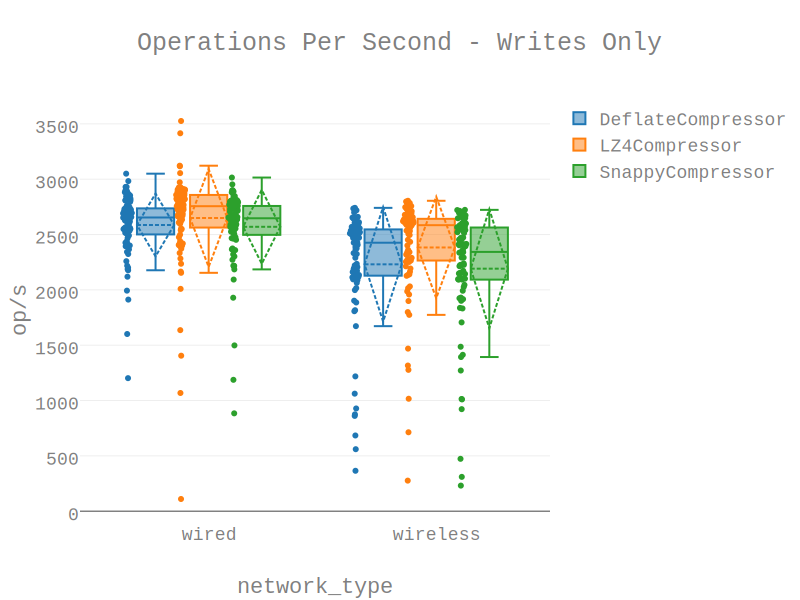
\includegraphics[width=7cm]{Figures/figures-cs1_fig1.pdf}

\caption{Varying Compression Methods: Writes}

\label{fig:res}
\end{figure}
	The above box plot shows the effect of varying compression strategies for a given configuration on a pure write load as load-tested through the cassandra-stress module.  In the left, wireless 802.11 links were used.  On the right, wired Ethernet links were used.  A one-way analysis-of-variance (ANOVA) may be able to test whether there is a significant differential between either of these two means, but from visual inspection, one could say that for a given configuration and a write-heavy load, varying the compression strategy does not have a large effect on performance as far as writes per second.
\begin{figure}[h]
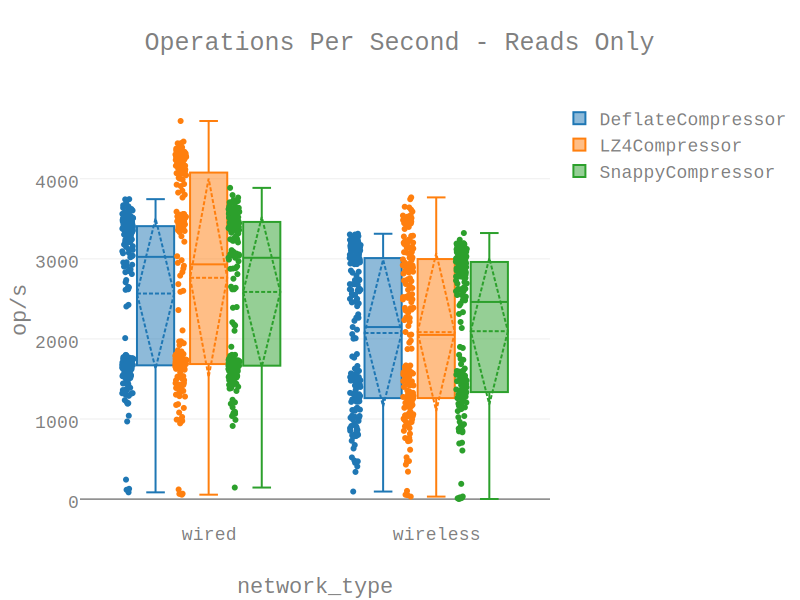
\includegraphics[width=7cm]{Figures/figures-cs1_fig2.pdf}

\caption{Varying Compression Methods: Reads}

\label{fig:res}
\end{figure}
	To represent a read-heavy load, a pure read load was put through cassandra-stress, varying both compression strategies and wireless versus wired link nature.  In the wired domain (right), a hierarchy seems to emerge.  The LZ4 compression algorithm renders the most reads per second, followed by the Snappy compression algorithm, and finally the Deflation compression algorithm.  This correlates with the expectations put forth by the manual, as the selection in compression algorithms represents a trade-off between speed (operations per second) and compression effectiveness (storage in bytes) for the user.  Such a hierarchy does not seem to emerge from the wireless links, but there is no known explanation for this at this time.  Increased variation is not unexpected, perhaps due to \gls{ism} band interference, but one would expect the means to follow a similar pattern.  A series or regressions or multi-factor \gls{anova} test could be utilized to see if the graph is deceiving and the means truly are significantly different, but is not merited at this time.

\begin{figure}[h]
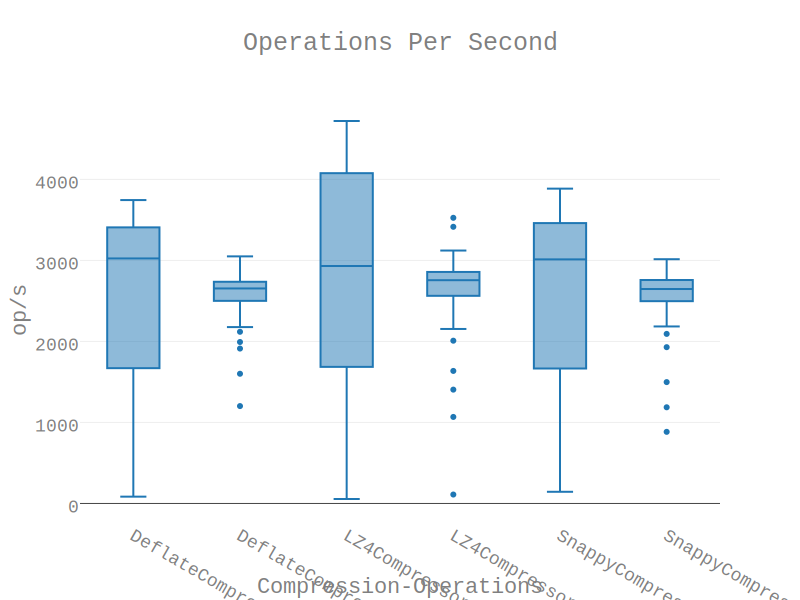
\includegraphics[width=7cm]{Figures/figures-cs1_fig3.pdf}

\caption{Compression Methods Sorted by Best Performance: Wired \gls{lan} Case}

\label{fig:res}
\end{figure}
	The above box-plot shows, for wired, how performance can vary with respect to different compression strategies and loads.  For reads, the compression strategy hierarchy seems to correlate with what is expected from reading the manual: the LZ4 algorithm renders highest performance in operations per second, followed by the Snappy algorithm, then the Deflate algorithm.  For writes, the hierarchy continues but is less pronounced.  

\begin{figure}[h]
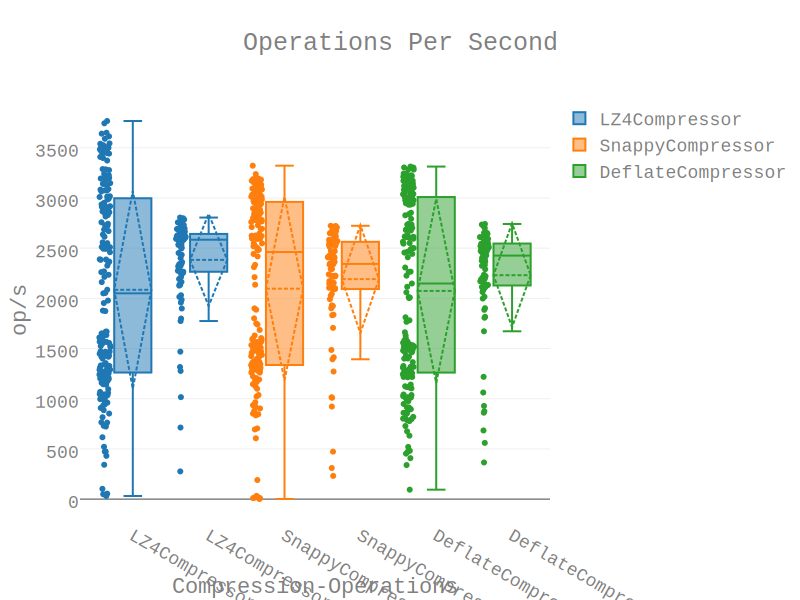
\includegraphics[width=7cm]{Figures/figures-cs1_fig4.pdf}

\caption{Compression Methods Sorted by Best Performance: Wireless \gls{lan} Case}

\label{fig:res}
\end{figure}

	For the wireless links, the LZ4 algorithm seems to remain the highest performer, but the Deflate and Snappy algorithms seem to exchange places in the hierarchy, both for reads and for writes.  The means, shown as the dashed horizontal lines are very close together on both counts, so a hypothesis that the switch is not significant may be of merit.  The main thing that this graph shows is that at least in one test, the wireless links allowed for reasonably similar performance levels across compression strategies and loads.  To a potential application in the \gls{iot} domain, this may imply that one is not sacrificing much in the manner of operations per second by configuring Cassandra to employ a more effective compression strategy, such as the Deflate algorithm.


